\documentclass[12pt, letter]{article}

%% Class name and Assignment number
%%
\newcommand{\courseName}{Introduction~to~Deep~Learning~for~Computer~Vision}
\newcommand{\assignName}{Assignment~3:~Simple~Linear~Classifier II}

%% Packages
\usepackage{amsmath,amsfonts,amssymb,amsthm,dsfont}
\usepackage{graphicx}
\usepackage[bookmarks=false]{hyperref}
\usepackage{color}
\usepackage{lipsum}

%% Paper format
\usepackage{geometry}
\geometry{
    letterpaper,
    %% total={216mm,279mm}, %< NSERC size
    margin=2.00cm,     %< default
    %% margin=1.87cm,       %< NSERC tightest
}

%% Headers and footers
\usepackage[explicit]{titlesec}
\newpagestyle{titlesec_assignment}{
  \sethead{\courseName}{}{\assignName}\setfoot{}{\thepage}{}
  \headrule
  %% \footrule
}

\begin{document}

%% Set header and footer
\pagestyle{titlesec_assignment}

%% Title
\title{\courseName\\\assignName}
\author{Paul Molina-Plant}
\maketitle

\abstract{TODO}

\pagebreak

\section{Derivation of the gradient for cross entropy}
\subsection{The cross entropy function}
\begin{equation}
  L_i = - log \frac{\sum_jt_{ij}e^{s_{ij}}}{\sum_ke^{s_{ik}}}
\end{equation}
I assume $log$ base $e$ for (1).
\begin{equation}
  t_{ij} = \delta_{ij} =
  \begin{cases}
    1 & j = y_i \\
    0 & j \ne y_i
  \end{cases}
\end{equation}
Softmax $P_{ij}$
\begin{equation}
  P_{ij} = \frac{e^{s_{ij}}}{\sum_{k}e^{s_{ik}}}
\end{equation}
Among the $k$ classes, $j = y_{i}$ for exactly one of them. Therefore, we can
ignore the other $k-1$ terms in the sum of (1).
\begin{equation}
  L_i = - ln \frac{e^{s_{ij}}}{\sum_k{e^{s_{ik}}}} = -ln P_{ij}
\end{equation}
\subsection{Gradient of $W$}
Computing the gradient $\frac{\partial L_i}{\partial W}$ via chain rule.
\begin{equation}\nonumber
  \frac{\partial L_i}{\partial W} =
  \frac{\partial L_i}{\partial P_{ij}} \frac{\partial P_{ij}}{\partial s_{ij}} \frac{\partial s_{ij}}{\partial W}
\end{equation}
Linear classifier $f(x_i, W) = s_{ij}$.
\begin{equation}
  s_{ij} = Wx_i + b_i
\end{equation}
The partial derivative of $s_{ij}$ wrt $W$ is nonzero when $j=y_i$
and zero everywhere else. This condition is expressed with $\delta_{ij}$ (2).
\begin{equation}\nonumber
  \frac{\partial s_{ij}}{\partial W} = \delta_{ij} x_i
\end{equation}
The partial derivative of $P_{ij}$ (3) wrt $W$ by applying the chain rule.
\begin{equation}\nonumber
\begin{split}
  \frac{\partial P_{ij}}{\partial W}& = \frac{\partial}{\partial W}\frac{e^{s_{ij}}}{\sum_ke^{s_{ik}}} = \frac{\delta_{ij}x_ie^{s_{ij}}-e^{s_{ij}}x_ie^{s_{ij}}}{\left(\sum_ke^{s_{ik}}\right)^2}\\
  & = \left(\frac{e^{s_{ij}}}{\sum_ke^{s_{ik}}}\right)\left(\frac{\delta_{ij}x_i\sum_ke^{s_{ik}}-x_ie^{s_{ij}}}{\sum_ke^{s_{ik}}}\right)\\
  & = P_{ij} (\delta_{ij}x_i - P_{ij}x_i) \\
  & = P_{ij}x_i(\delta_{ij} - P_{ij})
\end{split}
\end{equation}
Finally the partial derivative of $L_i$ (4) wrt $W$.
\begin{equation}
\begin{split}
  \frac{\partial L_i}{\partial W}& = \frac{\partial}{\partial W}\left(-lnP_{ij}\right)\\
  & = -\frac{1}{P_{ij}} P_{ij}x_i(\delta_{ij} - P_{ij})\\
  & = (\delta_{ij} - P_{ij}) x_i
\end{split}
\end{equation}
\pagebreak
\subsection{Gradient of $b_i$}
Computing the gradient $\frac{\partial L_i}{\partial b_i}$ via chain rule.
\begin{equation}\nonumber
  \frac{\partial L_i}{\partial b_i} =
  \frac{\partial L_i}{\partial P_{ij}} \frac{\partial P_{ij}}{\partial s_{ij}} \frac{\partial s_{ij}}{\partial b_i}
\end{equation}
The partial derivative of $s_{ij}$ (5) wrt $b_i$ is nonzero when $j=y_i$
and zero everywhere else. This condition is expressed with $\delta_{ij}$ (2).
\begin{equation}\nonumber
  \frac{\partial s_{ij}}{\partial W} = \delta_{ij}
\end{equation}
The partial derivative of $P_{ij}$ (3) wrt $b_i$ by applying the chain rule.
\begin{equation}\nonumber
  \frac{\partial P_{ij}}{\partial b_i} = \frac{\partial}{\partial W}\frac{e^{s_{ij}}}{\sum_ke^{s_{ik}}} = \frac{-e^{s_{ij}}e^{s_{ij}}}{\left(\sum_ke^{s_{ik}}\right)^2} = -P_{ij}^2
\end{equation}
Finally the partial derivative of $L_i$ (4) wrt $b_i$.
\begin{equation}
\begin{split}
  \frac{\partial L_i}{\partial b_i}& = \frac{\partial}{\partial b_i}\left(-lnP_{ij}\right)\\
  & = -\frac{1}{P_{ij}} (-P_{ij}^2) \\
  & = P_{ij}
\end{split}
\end{equation}


\pagebreak

Example Section.

\subsection{Example Subsection}

Example Sub Section.

\paragraph{Example paragraph.}


\subsection{Example  Equation}

This is how a equation looks like.
\begin{equation}
  y = a x^2 + b x + c
  \;\;,
\end{equation}
where an inline equation looks like $a=b$.

\subsection{Example  Figure}

To put a figure, you can do as shown in Fig.~\ref{fig:eg}.
%%
\begin{figure}
  \centering
  \rule{2cm}{2cm} % Replace this with below, and your actual figure
  %% 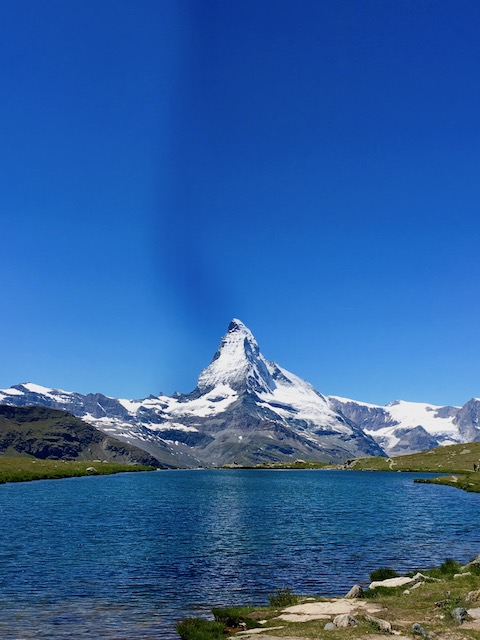
\includegraphics[width=0.4 \textwidth]{input.jpg}
  \caption{Example caption.}
  \label{fig:eg}
\end{figure}

\end{document}


%%% Local Variables:
%%% mode: latex
%%% TeX-master: t
%%% End:
